\documentclass[11pt]{article}
\usepackage{amssymb, amsthm, amsmath}
\usepackage{graphicx}
\usepackage{bm}
\usepackage{doublespace}
\usepackage[authoryear]{natbib}
\usepackage{times}
\usepackage{multirow}


\newcommand{\bbeta}{\bm{\beta}}
\newcommand{\beps}{\bm{\epsilon}}
\newcommand{\bX}{\bm{X}}
\newcommand{\bY}{\bm{Y}}
\newcommand{\bI}{\bm{I}}


\linespread{1} 
\topmargin= -.5in \oddsidemargin= 0in
\evensidemargin= 0in \textwidth=6.5in \textheight=9in

\begin{document}

\begin{center}
	{\Large {\bf ST 758 Project 1}}\\ \vspace{12pt}
	{\large {\bf Jessica Miller}}\\ \vspace{12pt}
	Oct. 25, 2016
	\vspace{5mm}
	\vspace{5mm}
\end{center}

\begin{flushleft}
	In this assignment, I studied the estimation of parameter values for the Ising model. In order to simplify the computations, which are slow for large n, I identified the following methods.
	\newline
	\newline
	Firstly, I realized that \(J_{ij}\) is a Toeplitz matrix. The \(\beta\) values for each model form the off-diagonals, the diagonal is zero, and the rest of the entries are zero. Thus the matrix is Toeplitz and sparse. Recognizing this makes the first multiplication and sum of the Hamilton function faster to compute.
	\newline
	\newline
	Secondly, I investigated the \(C\) function in the denominator of the probability mass function. The summation of \(C\) is supposed to be over all the \(2^{24}\) possibilities of \(\sigma\). However, \(\sigma\) is binary, \(\sigma \in (-1,1) \). Thus, the very largest \(C\) can be is the sum of all the times \(\sigma\) is equal to 1. The rest of the possibilities would cancel out. Thus, we reduce the size of \(C\) tremendously, making the probability mass function much quicker to compute.
	\newline
	\newline
	After writing the functions in R for each model, I initialized values of \(\beta\) and \(\alpha\) to input to each function. Also, I kept \(h\) constant at \(h=1\). For Model 1, I let \(\beta \in (0.25, 0.5, 1, 1.5, 2, 3, 5)\). Models 2 and 3 followed similarly, with each \(\beta_j\) equaling one of the values used for Model 1. For the exponential model, I let \(\alpha\) be each of the above values as well.
	\newline
	\newline
	The parameter values that maximized the likelihood for \(\beta\) were (.483, .320, .239) and the \(\alpha\) value was .266.
\end{flushleft}

\begin{flushleft}
	In Figure \ref{e:max} and Figure \ref{f:mean} below, we can see the contour plots for the parameters.
\end{flushleft}

\begin{figure}[h]\begin{center}
		\caption{The \(\beta\)s in Model 1 are shown.}\label{e:max}
		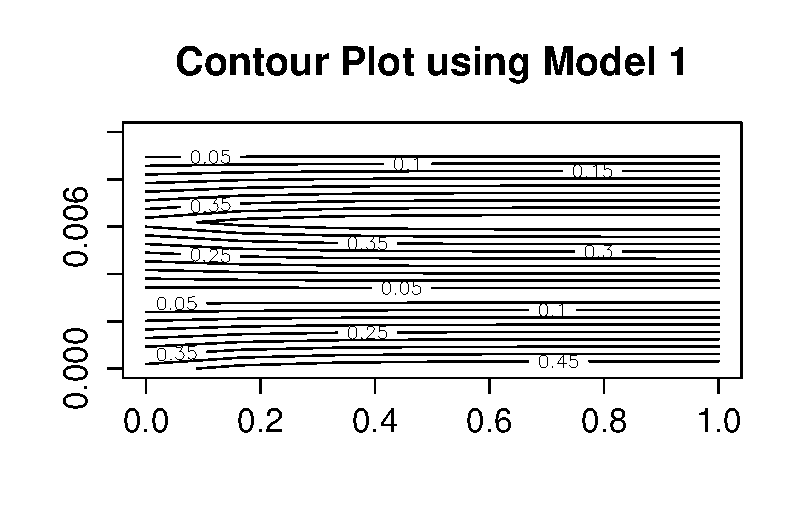
\includegraphics[width=.8\textwidth]{proj1plot2}	
	\end{center}\end{figure}

\begin{figure}[h]\begin{center}
		\caption{The \(\alpha\)s in the exponential model are shown.}\label{f:mean}
		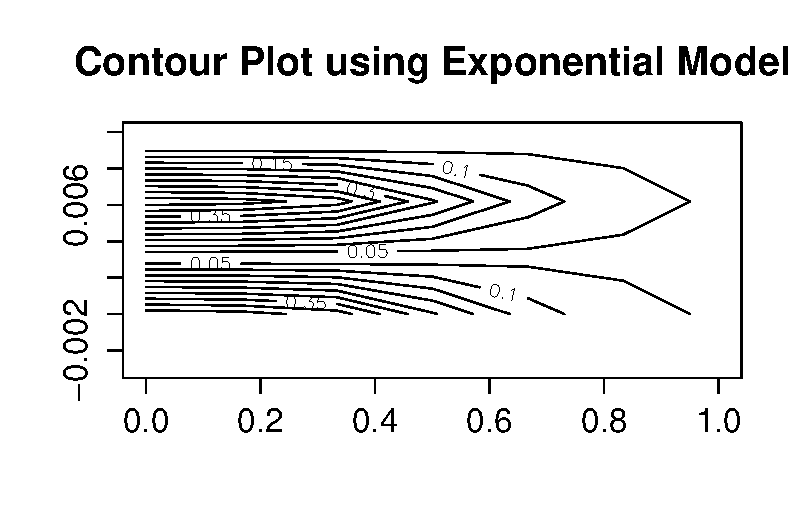
\includegraphics[width=.8\textwidth]{proj1plot1}	
	\end{center}\end{figure}
	


\end{document}
